% fig7_21.tex — 7-23: 旋转圆盘 + 弹簧 + 小球
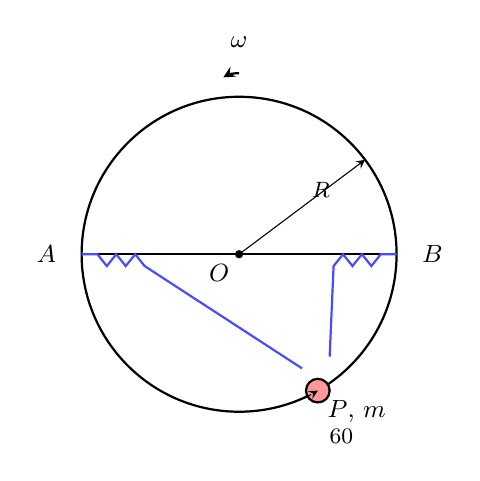
\begin{tikzpicture}[font=\small,>=stealth]
  % 圆盘（俯视图）
  \draw[thick] (0,0) circle (2);
  % 圆心 O
  \fill (0,0) circle (1.5pt);
  \node[below left] at (0,0) {$O$};
  % 直径 AB
  \draw[thick] (-2,0) -- (2,0);
  \node[left] at (-2.2,0) {$A$};
  \node[right] at (2.2,0) {$B$};
  % 标注圆盘半径
  \draw[->] (0,0) -- (1.6,1.2) node[midway,above right,font=\footnotesize] {$R$};
  % 弹簧1：从A到小球P
  % P在圆弧AP=60°处，即P在 (R*cos(-60°), R*sin(-60°)) = (R/2, -R√3/2)
  % 即 (1, -1.732)
  \draw[thick,blue!70] (-2,0) -- ++(0.2,0)
    foreach \i in {1,...,5}{
      -- ++(0.12,{(-1)^\i*0.15})
    } -- (0.8,-1.45);
  % 弹簧2：从B到小球P
  \draw[thick,blue!70] (2,0) -- ++(-0.2,0)
    foreach \i in {1,...,5}{
      -- ++(-0.12,{(-1)^\i*0.15})
    } -- (1.15,-1.3);
  % 小球 P
  \draw[thick,fill=red!40] (1,-1.732) circle (0.15);
  \node[below right] at (1,-1.732) {$P$, $m$};
  % 圆弧AP标注
  \draw[->,dashed] (0,-2) arc[start angle=270,end angle=300,x radius=2,y radius=2];
  \node[below,font=\footnotesize] at (1.3,-2.1) {$60°$};
  % 旋转箭头
  \draw[->,thick] (0,2.3) arc[start angle=90,end angle=120,x radius=0.4,y radius=0.4];
  \node[above] at (0,2.5) {$\omega$};
\end{tikzpicture}
